\documentclass[a4paper,12pt]{article}

\usepackage{amsmath,amssymb,amsfonts,gensymb,mathtext,enumerate,float,cite}
\usepackage[T2A]{fontenc}
\usepackage[utf8]{inputenc}
\usepackage[english,russian]{babel}
\usepackage{indentfirst}
\usepackage[unicode=true]{hyperref}
\usepackage{multirow}
\usepackage{array}	
\usepackage[dvips]{graphicx}
\usepackage{xymtexpdf}
\usepackage{caption}
\usepackage{cmap}
\graphicspath{{images/}}
\usepackage{diagbox}  % Add this to your preamble
\usepackage{multirow}
\usepackage{array}



\usepackage{setspace}
% полуторный интервал
\onehalfspacing
\usepackage[12pt]{extsizes}

\hypersetup{
pdfborder={0 0 0},
pdfauthor={Khaibrakhmanov Artur Ilnurovich},
pdftitle={Thesis},
}

\usepackage{geometry}\geometry{left=2cm}
\geometry{right=2cm}
\geometry{top=2cm}
\geometry{bottom=2.5cm}

%\numberwithin{equation}{section}
%\numberwithin{figure}{section}
%\numberwithin{table}{section}

\setcounter{tocdepth}{4}
\setcounter{secnumdepth}{4}

\RequirePackage{caption}
\usepackage[labelsep=period]{caption}
%\DeclareCaptionLabelSeparator{defffis}{ -- }
\captionsetup{justification=centering}%,labelsep=defffis}
\usepackage{subfigure}
\usepackage{subcaption}
\renewcommand{\thesubfigure}{(\asbuk{subfigure})}
\begin{document}
\righthyphenmin=20
\renewcommand{\figurename}{Рисунок}
\setcounter{page}{1}
\renewcommand{\contentsname}{Оглавление}

\begin{center}
\text{Химия}\\
\begin{Large}
\textbf{Решение проблемы фаз с помощью методов глубокого обучения в обратном пространстве}\\
\end{Large}
\text{Хайбрахманов Артур Ильнурович}\\
\text{Колпинский Сергей Викторович, Дмитриенко Артем Олегович}\\
\end{center}







\sloppy{
\subsection*{Аннотация}

Решение проблемы фаз является важной задачей рентгеноструктурного анализа, особенно актуальной для белковой кристаллографии ввиду отсутствия ab initio решений в этой области. Методы машинного обучения способны преодолеть данную задачу. Предлагается увеличивать разрешение дифракционной картины, предсказывая моделью машинного обучения дальние отражения по ближним, что позволит решить проблему фаз ab initio для биомолекул. В работе разработан генератор синтетических рентгенодифракционных данных, который может быть использован для решения прикладных задач методами ИИ, и пайплайн для проведения воспроизводимых экспериментов для решения задачи в рамках предложенной методологии. Также были разработаны модели FFT\_UNet и XRD\_Transformer, подходящие под специфику задачи; проведены их сравнительный анализ и интерпретация их работы с помощью GradCAM и связей внимания. Было показано и обосновано, что методы глубокого обучения способны считывать кристаллографические связи и законы в рентгенодифракционных данных, но их точности численного восстановления амплитуд структурных факторов не хватает для решения проблемы фаз в рамках предложенной методологии. 

\subsection*{Ключевые слова}
Рентгеновская дифракция, проблема фаз, нейронные сети, машинное обучение, структурный фактор, рентгеноструктурный анализ, трансформер

\subsection*{Введение}

Рентгеновская кристаллография является важнейшим инструментом определения трехмерных структур кристаллов. Этот метод позволяет получить бесценные сведения об атомных и молекулярных структурах кристаллов, что крайне важно для понимания свойств и функций материалов в различных областях, включая химию, биологию и материаловедение. Рентгеноструктурный анализ основан на упругом рассеянии монохроматического рентгеновского излучения на трехмерной регулярной решетке атомов твердого вещества, что приводит к интерференции рентгеновских лучей.

Дифракция в кристалле описывается как отражения от семейств параллельных кристаллографических плоскостей элементарной ячейки кристалла. Каждая точка дифракционной картины задается набором из индексов Миллера $h,k,l$. Любое отражение имеет математическое представление, известное как структурный фактор $F(h,k,l)$, зависящий от расположения и коэффициентов рассеяния всех
атомов в элементарной ячейке кристалла. Структура кристалла получается при расчете электронной плотности с помощью Фурье-преобразования: \[\rho(x, y, z) = V^*\sum_{h,k,l} F(h,k,l) exp[(-2\pi i (hx+ky+lz)],\] где $V^*$~-- объем элементарной обратной ячейки \cite{giro}. 

Структурный фактор является комплексной величиной, и её амплитуда  $|F(h,k,l)|$ легко определяется по результатам обычного рентгенодифракционного эксперимента как квадратный корень из зарегистрированной интенсивности дифрагированной волны, а информация о фазе теряется. Данная проблема получила название "проблема фаз". Без знания о фазе процесс восстановления распределения электронной плотности из дифракционных данных затруднен.

Проблема фаз давно является одной из главных задач рентгеновской кристаллографии. Для ее решения были разработаны традиционные методы, такие как прямые \cite{direct} и charge-flipping \cite{charge_flipping}, но они, как правило, ограничены атомным разрешением рентгенодифракционных данных. Эти методы требуют полного набора дифракционных пиков и часто требуют выращивания высококачественных образцов кристаллов, что может быть сложной задачей, особенно для слабо рассеивающих кристаллов или больших молекул, таких как белки \cite{protein_crystallography}. Для определения структур макромолекулярных соединений разработаны методы молекулярного замещения и изоморфного замещения, требующие дополнительную информацию --- знание о структуре белка с той же аминокислотной последовательностью или результаты рентгенодифракционных экспериментов той же структуры с добавлением тяжелых атомов, соответственно \cite{acta}. Таким образом, решение проблемы фаз является особенно актуальной задачей белковой кристаллографии из-за отсутствия ab initio решений. 

Применение машинного обучения в области рентгеновской дифракции лишь недавно зародилось и сейчас бурно развивается. Чаще всего авторы пытаются обойти решение проблемы фаз, предсказывая кристаллическую структуру из доступных экспериментальных данных. Так, были разработаны модели глубокого обучения, позволяющие миновать проблему фаз, работая напрямую с функцией Паттерсона, которые получаются из дифракционных данных, не требуя информации о фазах отражений \cite{patterson}. Эти модели представляют собой сверточные нейронные сети для предсказания распределения электронной плотности структуры по функции Паттерсона, демонстрируя многообещающие результаты на простых примерах дипептидов и подчеркивая потенциал для более широкого применения в белковой кристаллографии.

В недавней статье \cite{science} с помощью методов глубокого обучения авторы предприняли попытку решить проблему фаз. В качестве объектов предсказания они выбрали центросимметричные структуры, для которых фазы отражений принимают два возможных значения --- 0 и 1. Авторы презентовали нейронную сеть, представляющую собой бинарный классификатор из блоков трехмерных свёрток и многослойных перцептронов. Обучение проводилось на синтетических кристаллических молекулярных структурах. Этот подход продемонстрировал способность решать фазовую задачу с разрешением всего 2$\text{\AA}$, используя всего 10--20$\text{\%}$ данных, требуемых традиционными методами. Также в работе реализована идея phase recycling~--- исходные данные прогоняются несколько раз через модель, что увеличивает точность классификации. Таким образом, впервые был продемонстрирован потенциал машинного обучения для решения проблемы фаз, но только для центросимметричных структур.

На основе методов глубокого обучения были также предложены решения аналогичной задачи в физике, особенно в области когерентной безлинзовой микроскопии. В обзорной статье \cite{review_physics} выделяются три подхода: DL-post-processing, где уточняются «плохие фазы», полученные из исходных интенсивностей; DL-in-processing, в котором нейронная сеть используется для непосредственного расчета фаз из интенсивностей; и DL-pre-processing, при котором обученная модель повышает разрешение микроскопического изображения, а фазы из полученного изображения определяются детерминированными методами. Однако, в кристаллографии дифракционные данные имеют гораздо меньшее разрешение, чем в когерентной микроскопии, что исключает возможность прямого применения существующих решений.

Таким образом, решение фазовой задачи белковой кристаллографии является актуальной задачей, нерешаемой рутинными методами. Инструменты на основе методов глубокого обучения способны преодолеть ограничения традиционных подходов, позволяя определять кристаллические структуры на основе ограниченных данных с низким разрешением. По мере развития исследований в этой области, вероятно, алгоритмы глубокого обучения станут незаменимым инструментом в области кристаллографии, облегчая решение сложных структур, которые ранее были неразрешимыми. Таким образом, разработка методов решения проблемы фаз с помощью ИИ является целью работы. 

\subsection*{Данные}

Было разработано программное обеспечение, позволяющие генерировать рентгенодифракционные данные случайных органических структур (\url{github.com/blackwood168/xrd_simulator}). С помощью библиотеки CCTBX (Computational Crystallography Toolbox \cite{cctbx}) создаются кристаллические решетки, в которых случайным образом расставлены атомы, и рассчитываются структурные факторы. Также генератор поддерживает последующий расчет данных рентгеновской порошковой дифракции. Так, можно получить достоверные дифрактограммы синтетических структур, в которых реализована профильная функция Псевдо-Войдта и аксиальная расходимость пучка. Данный генератор может быть полезен для генерации рентгенодифракционных синтетических данных для использования в различных прикладных задачах машинного обучения в данной области.

Начальное обучение моделей глубокого обучения было решено проводить на синтетических данных, которые могут быть рассчитаны с помощью разработанного генератора. Высокое разрешение выбрано 0.8 Å, низкое --- 1.5 Å. Рассматриваются только симметрийно независимые отражения, так как данные о симметрии известны и без решения проблемы фаз. Так как общее количество симметрийно независимых отражений структур (для ячеек одного размера) зависит от сингонии (класса кристаллических решеток), все структуры в данных были моноклинными. Таков выбор неслучаен --- моноклинные группы симметрии являются одними из наболее распространенными для белковых структур в базе данных белков (\url{rcsb.org/stats/distribution-space-group}). Соответственно группы симметрии --- P$2_1$, C2. Типы атомов --- C, N, O, Cl; число симметрийно независимых атомов 10--30. Для обучения были сгенерированы 400.000, 100.000 и 100.000 структур для тренировочной, валидационной и тестовой выборок, соответственно.

Также в работе использовались реальные моноклинные молекулярные структуры малых молекул из Кембриджского Банка Структурных Данных \cite{csd}, для которых были расчитаны дифракционные отражения. 10.000 структур использовались для дообучения моделей на реальных структурах, 2000 --- были отложены для тестирования.

Так как отражения являются точками обратного пространства, каждое из них можно однозначно описать индексами Миллера (h,k,l). Тогда дифракционную картину можно описать трехмерным тензором, в котором записаны данные каждого отражения. Размер тензора был выбран (26,18,23) --- в матрицу такого размера помещаются все отражения для самой большой моноклинной структуры из синтетических данных. Соответственно для обучения данные об отражениях были помещены в тензор, в позициях (h,k,l) соответственно, где дифракционные максимумы отсутствуют --- стоят нули.

Для выполнения работы валидным является предсказание как интенсивности, так и амплитуды структурных факторов ($|F| = \sqrt{I}$). Типичные распределения этих данных для сгенерированных структур представлены на рис. \ref{F_dist}. Как можно заметить, распределение амплитуд больше похоже на стандартное, поэтому именно амплитуды были выбраны для решения задачи. Дифракционные данные также были отнормированы в диапазон 0-1.

\begin{figure*}[ht!]
            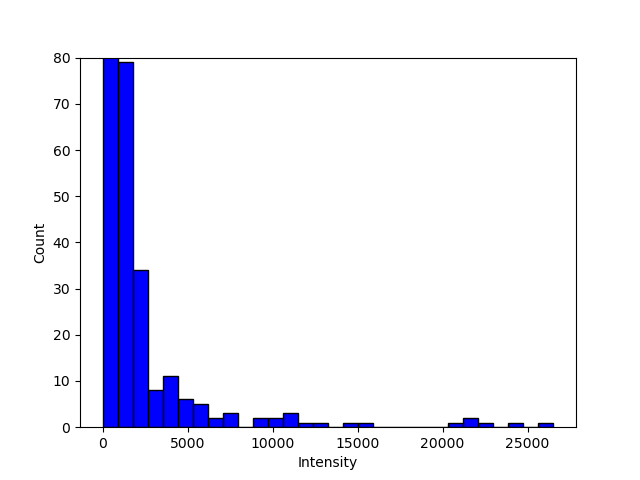
\includegraphics[width=.5\textwidth]{F2_distribution.png}\hfill
            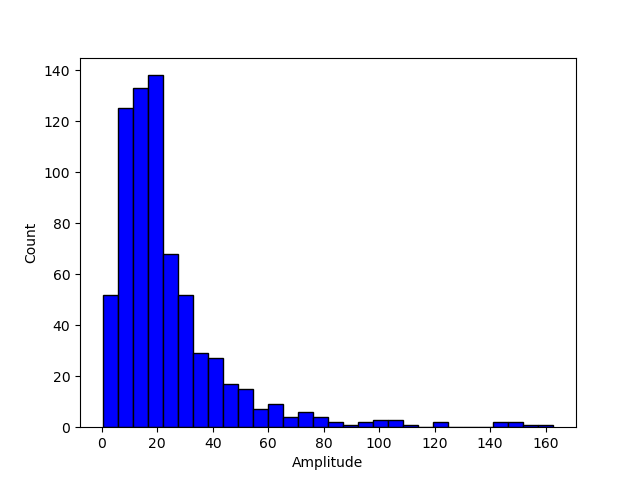
\includegraphics[width=.5\textwidth]{F_distribution.png}
            \caption{Типичные распределения интенсивностей (слева) и амплитуд (справа) дифракционной картины}
            \label{F_dist}
\end{figure*}

Основная же сложность работать с чистыми амплитудами структурных факторов --- то есть с точками в обратном пространстве --- заключается в том, что данные не являются локально связанными, как изображения (рис. \ref{locally}). Это вносит специфику в данную задачу и создает трудности, так как типичные архитектуры моделей для работы с трехмерными данными, например, видео или медицинскими данными \cite{mrt} могут не сработать.

\begin{figure*}[ht!]
            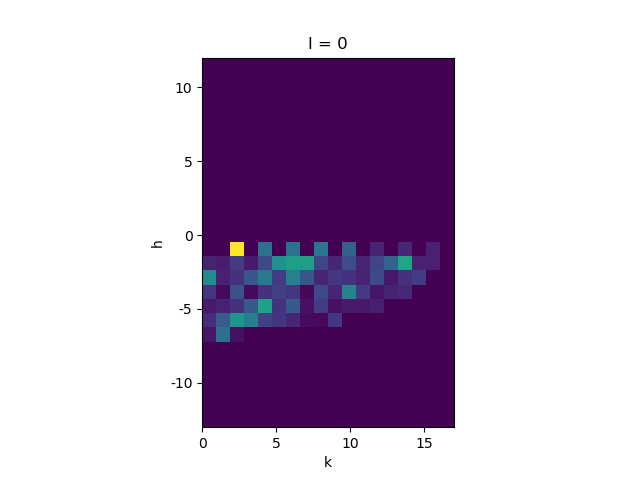
\includegraphics[width=.3\textwidth]{hk_plane_l_0.png}\hfill
            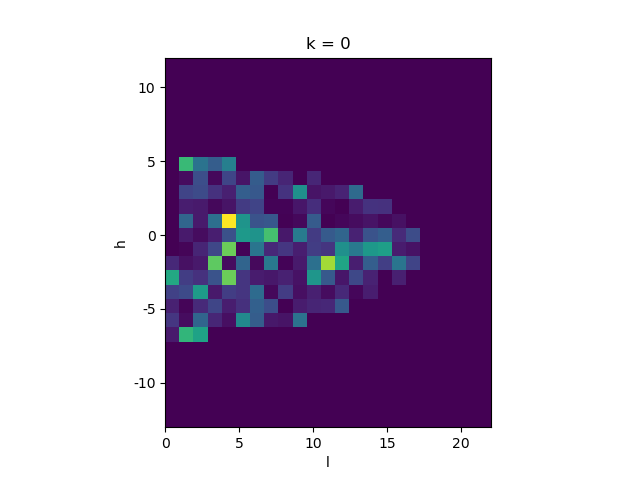
\includegraphics[width=.3\textwidth]{hl_plane_k_0.png}\hfill
            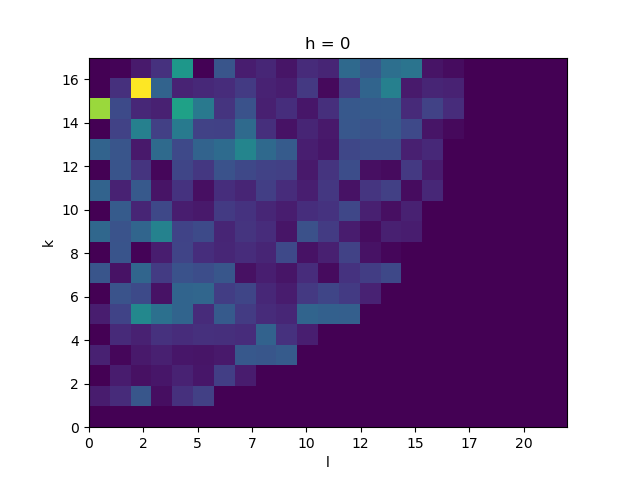
\includegraphics[width=.3\textwidth]{kl_plane_h_0.png}
            \caption{Типичные сечения тензора отражений для реальных структур из CSD}
            \label{locally}
\end{figure*}


\subsection*{Методология}

В работе было предложено предсказывать амплитуды дифракционных отражений белков, которые нельзя получить из эксперимента, по известным из того же эксперимента. После предсказания достаточного количество рефлексов, разрешения должно хватить для определения фаз и расчета электронной плотности одним из рутинных ab initio методов, в качестве которого был выбран SHELX \cite{shelx}.

Таким образом, задача сводится к восстановлению трехмерного тензора. Inference моделей глубокого обучения должен выглядеть следующим образом: на вход подается тензор с рентгенодифракционными экспериментальными данными, на выходе должен быть тензор с дополнительными интенсивностями. В ходе обучения планируется научить модель восстанавливать тензор отражений по данным малых органических молекул. Для этого будут обнулены интенсивности дальних отражений так, чтобы длина разрешения полученной дифракционной картины соответствовала типичному разрешению белковых соединений (1.5 Å).

В качестве baseline была обучена модель UNet, адаптированная для трехмерных тензоров (рис. \ref{unet}). Данная модель выбрана потому что она хорошо себя проявляет в простейших задачах Super Resolution, однако в данной задаче она не достигнет высокой точности из-за локальной несвязанности рентгенодифракционных данных. 

\begin{figure}[H]
    \centering
    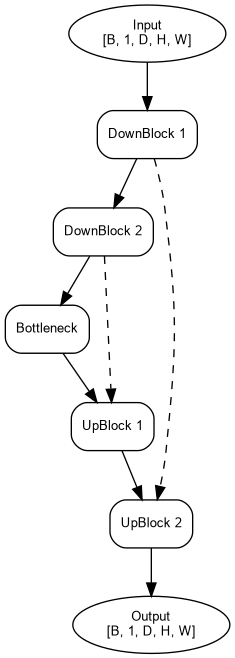
\includegraphics[width=0.25\textwidth]{mini_unet_architecture.png}
    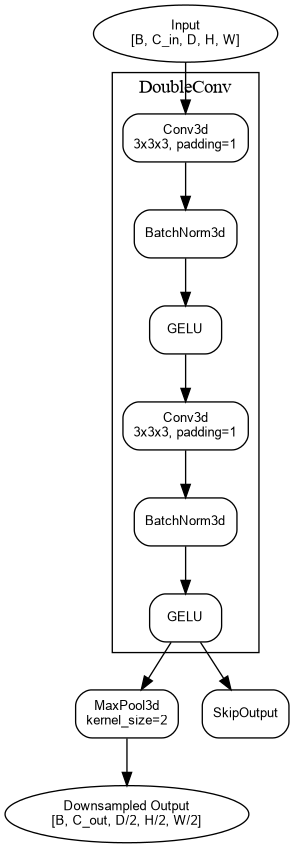
\includegraphics[width=0.25\textwidth]{downblock_architecture.png}
    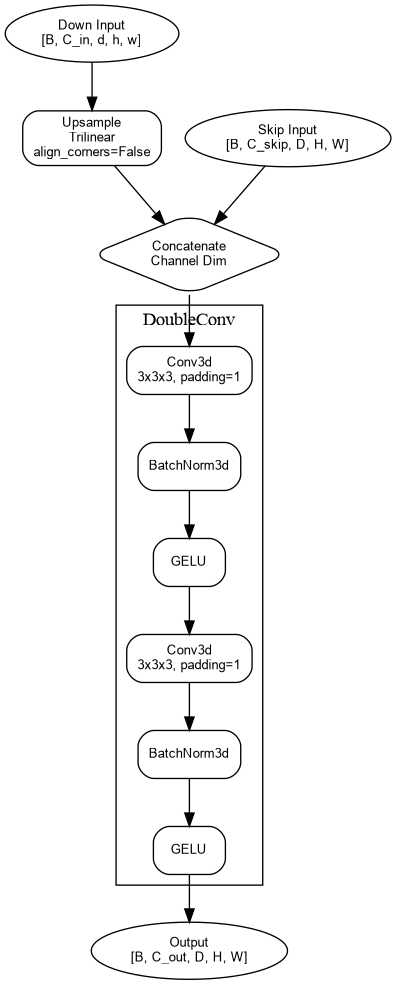
\includegraphics[width=0.3\textwidth]{upblock_architecture.png}
    \caption{Схемы архитектуры модели UNet (слева) и её DownBlock(посередине) и UpBlock(справа)}
    \label{unet}
\end{figure}

Также была разработана и обучена UNet-like модель с кастомными слоями, содержащими Фурье-преобразование (рис. \ref{fft_unet}). Данный подход был продемонстрирован в работе \cite{fft} при работе с дифракционными данными и он является многообещающим и для нашей задачи, поскольку при переходе в прямое пространство наши данные являются локально связанными.


\begin{figure}[H]
    \centering
    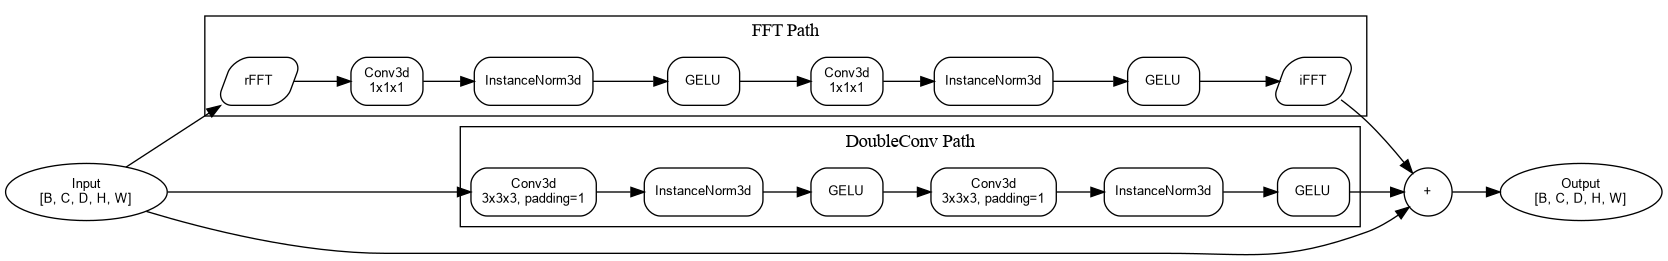
\includegraphics[width=0.8\textwidth]{resf_block_architecture.png}
    \caption*{(a) Кастомный слой с Фурье-преобразованием}
    
    \vspace{1em}
    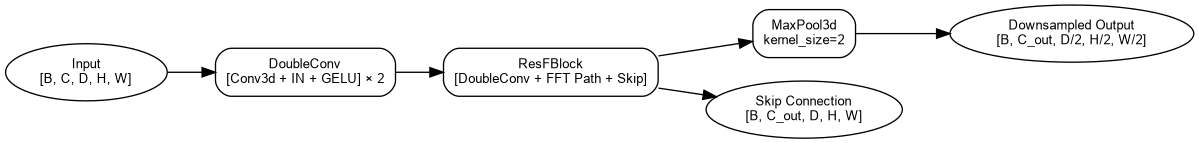
\includegraphics[width=0.8\textwidth]{fft_down_block_architecture.png}
    \caption*{(b) DownBlock}
    
    \vspace{1em}
    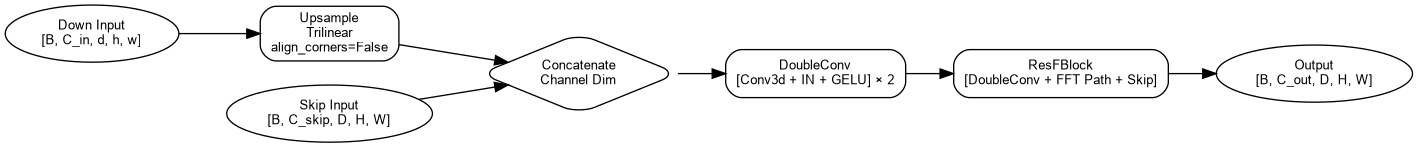
\includegraphics[width=0.8\textwidth]{fft_up_block_architecture.png}
    \caption*{(c) UpBlock}
    
    \caption{Кастомная FFT\_UNet модель и её основные блоки}
    \label{fft_unet}
\end{figure}

Поскольку тензоры дифракционных картин не являются локально связанными, актуально использование механизма внимания. Он позволит модели находить связи между не близколежащими отражениями. Так, был разработан трансформер XRD\_Transformer для нашей задачи (рис. \ref{XRDTrans}). 

\begin{figure}[H]
    \centering
    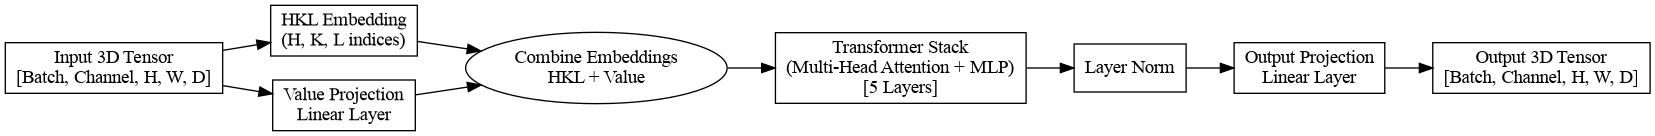
\includegraphics[width=1\textwidth]{transformer.png}
    \caption{Архитектура модели XRD\_Transformer}
    \label{XRDTrans}
\end{figure}

В модели формируется единый эмбеддинг из эмбеддинга индексов Миллера (h,k,l) и проекции значений амплитуды отражений. Затем эмбеддинг подается в 5 слоев трансформера, которые состоят из Multi-Head Attention и полносвязного слоев. Затем после нормализации и обратного проецирования в исходное пространство получается восстановленный тензор дифракционной картины.

Так как нам известны все возможные значения индексов Миллера (h,k,l) эмбеддинг (рис. \ref{hklembed}) формируется следующим образом: каждый индекс кодируется one-hot энкодингом. Затем каждый вектор с помощью обучаемого линейного слоя проецируется к размерности embed\_dim/3; после конкатенации получается эмбеддинг позиции отражения размерности embed\_dim. Также в модели реализована возможность эмбеддинга через полносвязный слой, который проецирует позицию (h,k,l) сразу в вектор эмбеддинга, однако она не использовалась при обучении модели, так как первый способ является более физическим для нашей задачи, поскольку мы используем только симметрийно независимые отражения.


\begin{figure}[H]
    \centering
    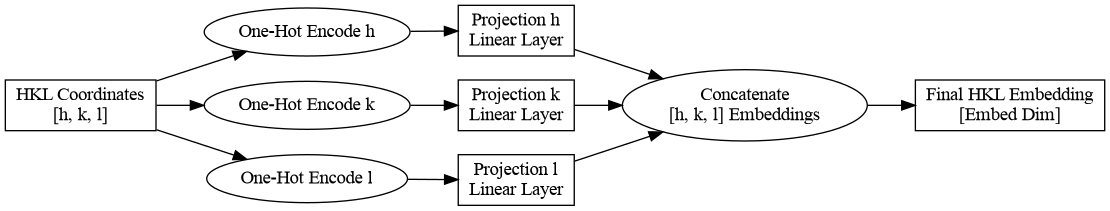
\includegraphics[width=1\textwidth]{hkl_embedding_process.png}
    \caption{Схема формирования эмбеддинга HKL}
    \label{hklembed}
\end{figure}

В ходе выполнения работы также предложен постпроцессинг, включающий в себя учёт систематических погасаний --- "зануления" некоторых значений интенсивностей, что определяется симметрией структуры; в ходе обучения происходит явное восстановления части тензора, которую не нужно предсказывать.

Для обучения моделей UNet и FFT\_UNet использовался оптимизатор Adam с планировщиком plateau scheduler (обучение: learning rate = 0.01, factor = 0.1; дообучение: learning rate = 0.0001, factor = 0.5); для XRD\_Transformer --- оптимизатор AdamW с планировщиком cosine annealing (обучение: learning rate = 0.01; дообучение: learning rate = 0.0001).

В качестве функции потерь была выбрана среднеквадратичная ошибка, минимизация которой должна приводить к восстановлению тензора рентгеновских отражений. В качестве метрики для анализа используется R-фактор: $R = \frac{\sum |F_{obs} - F_{calc}|}{\sum |F_{obs}|}$, где $|F_{obs}|$ --- экспериментальные структурные факторы, $|F_{calc}|$ --- рассчитанные структурные факторы. R-фактор является общепринятым стандартом в кристаллографическом сообществе для оценки качества структурных моделей. Нулевое значение R-фактора отвечает идеальному соответствию между данными модельной структуры и экспериментальными данными.

Также в качестве метрики рассматривался SSIM, однако эксперименты с ним в качестве добавки к функции потери привели к более низкому качеству восстановления модели с точки зрения R-фактора. Данный результат можно объяснить отсутствием локальности наших данных.

Эффективность предсказания обученных моделей глубокого обучения проверялась на тестовой части синтетического датасета, а также тестовой части рентгенодифракционных данных моноклинных структур из CSD.


\subsection*{Результаты}




% %csd do
% \begin{table}[H]
% \centering
% \begin{tabular}{|c|c|c|c|} 
% \hline
% \diagbox{\textbf{Metric}}{\textbf{Model}} & \textbf{UNet} & \textbf{FFT\_UNet} & \textbf{XRD\_Transformer}  \\ 
% \hline
% \textbf{MSE}                              & 2,67E-03      & 3,73E-03                           & 3,31E-03                                   \\ 
% \hline
% \textbf{R}                                & 0,590         & 0,646                              & 0,581                                      \\
% \hline
% \end{tabular}
% \end{table}

% %csd posle
% \begin{table}[H]
% \centering
% \begin{tabular}{|c|c|c|c|} 
% \hline
% \diagbox{\textbf{Metric}}{\textbf{Model}} & \textbf{UNet} & \textbf{FFT\_UNet} & \textbf{XRD\_Transformer}  \\ 
% \hline
% \textbf{MSE}                              & 1,39E-03      & 1,20E-03           & 1,31E-03                   \\ 
% \hline
% \textbf{R}                                & 0,393         & 0,336              & 0,358                      \\
% \hline
% \end{tabular}
% \end{table}

% %100k do

% \begin{table}[H]
% \centering
% \begin{tabular}{|c|c|c|c|} 
% \hline
% \diagbox{\textbf{Metric}}{\textbf{Model}} & \textbf{UNet} & \textbf{FFT\_UNet} & \textbf{XRD\_Transformer}  \\ 
% \hline
% \textbf{MSE}                              & 3,34E-04      & 5,65E-04           & 2,75E-04                   \\ 
% \hline
% \textbf{R}                                & 0,477         & 0,726              & 0,346                      \\
% \hline
% \end{tabular}
% \end{table}

% %100k posle

% \begin{table}[H]
% \centering
% \begin{tabular}{|c|c|c|c|} 
% \hline
% \diagbox{\textbf{Metric}}{\textbf{Model}} & \textbf{UNet} & \textbf{FFT\_UNet} & \textbf{XRD\_Transformer}  \\ 
% \hline
% \textbf{MSE}                              & 6,27E-04      & 6,62E-04           & 6,36E-04                   \\ 
% \hline
% \textbf{R}                                & 0,632         & 0,619              & 0,615                      \\
% \hline
% \end{tabular}
% \end{table}

% %FFT-UNet

% \begin{table}[H]
% \centering
% \begin{tabular}{|l|l|l|} 
% \hline
% \diagbox{\textbf{Metric}}{\textbf{Dataset}} & \textbf{Synth} & \textbf{CSD}  \\ 
% \hline
% \textbf{Before, R}                   & 0,726          & 0,646         \\ 
% \hline
% \textbf{After, R}                    & 0,619          & 0,336         \\ 
% \hline
% $\Delta$, \%                         & 14,7           & 48,0          \\
% \hline
% \end{tabular}
% \end{table}

% %UNet

% \begin{table}[H]
% \centering
% \begin{tabular}{|l|l|l|} 
% \hline
% \diagbox{\textbf{Metric}}{\textbf{Dataset}} & \textbf{Synth} & \textbf{CSD}  \\ 
% \hline
% \textbf{Before, R}                   & 0,477          & 0,590         \\
% \hline
% \textbf{After, R}                    & 0,632          & 0,393         \\ 
% \hline
% $\Delta$, \%                         & -32,6          & 33,4          \\
% \hline
% \end{tabular}
% \end{table}

% %XRDtrans

% \begin{table}[H]
% \centering
% \begin{tabular}{|l|l|l|} 
% \hline
% \diagbox{\textbf{Metric}}{\textbf{Dataset}} & \textbf{Synth} & \textbf{CSD}  \\ 
% \hline
% \textbf{Before, R}                   & 0,346          & 0,581         \\ 
% \hline
% \textbf{After, R}                    & 0,615          & 0,358         \\ 
% \hline
% $\Delta$, \%                         & -77,9          & 38,4          \\
% \hline
% \end{tabular}
% \end{table}


В рамках данной работы был разработан пайплайн, позволяющий проводить воспроизводимые эксперименты по решению проблемы фаз с помощью предложенной методологии. (\url{github.com/blackwood168/xrd_phase_ml}). В нем реализовано обучение и тестирование моделей, а также inference на реальных массивах данных и структурах кристаллических соединений. В репозитории присутствуют маленькие датасеты из сгенерированных и реальных структур малых органических молекул. Также там представлены веса обученных в работе моделей. Воспроизводимость обучения обеспечивает фиксирование начальных значений генераторов случайных состояний.

\subsubsection*{Результаты обучения}

\begin{table}[H]
\caption{Эффективность моделей до и после дообучения на синтетическом и реальном датасете}
\label{doposle}
\centering
\footnotesize
\begin{tabular}{|l|l|l|l|} 
\hline
\textbf{Model} & \textbf{Metric} & \textbf{Synth} & \textbf{CSD}  \\ 
\hline
\multirow{3}{*}{UNet} 
& Before, R & 0.477 & 0.590 \\ 
& After, R  & 0.632 & 0.393 \\ 
& $\Delta$, \%       & -32.6 & 33.4  \\
\hline
\multirow{3}{*}{FFT\_UNet}
& Before, R & 0.726 & 0.646 \\ 
& After, R  & 0.619 & \textbf{0.336} \\ 
& $\Delta$, \%       & 14.7  & 48.0  \\
\hline
\multirow{3}{*}{XRD\_Transformer}
& Before, R & 0.346 & 0.581 \\ 
& After, R  & 0.615 & 0.358 \\ 
& $\Delta$, \%       & -77.9 & 38.4  \\
\hline
\end{tabular}
\end{table}

Было проведено обучение на синтетических данных и последующее дообучение на реальных. Сравнение R-фактора для моделей до и после дообучения представлено в таблице \ref{doposle}. После дообучение на реальных данных точность предсказания моделей увеличивается минимум в 1.5 раза, однако теряют в точности на синтетических данных, кроме кастомного UNet с Фурье-преобразованием. Лучшую точность имеет модель UNet\_FFT, от которой немного отстает трансформер. В сводной таблице \ref{svod} представлены значения метрик на реальных данных финальных моделей. Таким образом, UNet\_FFT занимает меньше видеопамяти, работает быстрее и достигает лучшей метрики на тестовых реальных данных.

\begin{table}[H]
\centering
\caption{Значения метрик на тестовом реальном наборе данных моделей после дообучения}
\label{svod}
\begin{tabular}{|c|c|c|c|} 
\hline
\diagbox{\textbf{Metric}}{\textbf{Model}} & \textbf{UNet} & \textbf{FFT\_UNet} & \textbf{XRD\_Transformer}  \\ 
\hline
MSE$\cdot10^{-3}$$                              & 1,39      & 1,20           & 1,31                   \\ 
\hline
R                                & 0,393         & \textbf{0,336}              & 0,358                      \\
\hline
\end{tabular}
\end{table}

\subsubsection*{Анализ моделей}

Также был проведен анализ полученных моделей. Для трансформера были построены карты внимания (рис. \ref{attention_maps}) при обработке одной из тестовых реальных структур, из которых видно, что модель в первых блоках имеет более рассеяное и равномерное внимание, что говорит о том, что сначала производится сбор общего контекста. В последующих блоках внимание становится более сфокусированным и локализованным, показывая, что модель учится выделять важные взаимосвязи. Также наблюдается способность модели связывать дальние отражения, что важно в нашей задаче. Более сильные связи наблюдается вдоль оси l; также можно заметить диагональные паттерны внимание, что соответствует систематическим погасаниям. Таким образом, можно сделать вывод, что модель научилась распрознавать кристаллографические закономерности.

\begin{figure}[H]
    \centering
    \includegraphics[width=1\textwidth]{all_attention_connections.png}
    \caption{Связи внимания в блоках трансформера}
    \label{attention_maps}
\end{figure}

Также был проведен анализ первого блока моделей UNet и FFT\_UNet с помощью GradCAM (рис. \ref{gradU}, \ref{gradFFT}). По паттерну для UNet можно замтетить, что модель обращает исключительное внимание на границы дифракционной картины низкого разрешения. Смущает, что высокие значения Attribution и Overlay достигаются во всем диапазоне вне дифракционной картины на входе. Паттерн же для FFT\_UNet кажется более разумным: Attribution и Overlay распространяются на входную картину и немного за неё, что показывает, что модель ищет информацию около границы дифракционной картины. Наиболее высокие значения внимания достигаются в высокоинтенсивной зоне, дальше от неё значения монотонно спадают.

\begin{figure}[H]
    \centering
    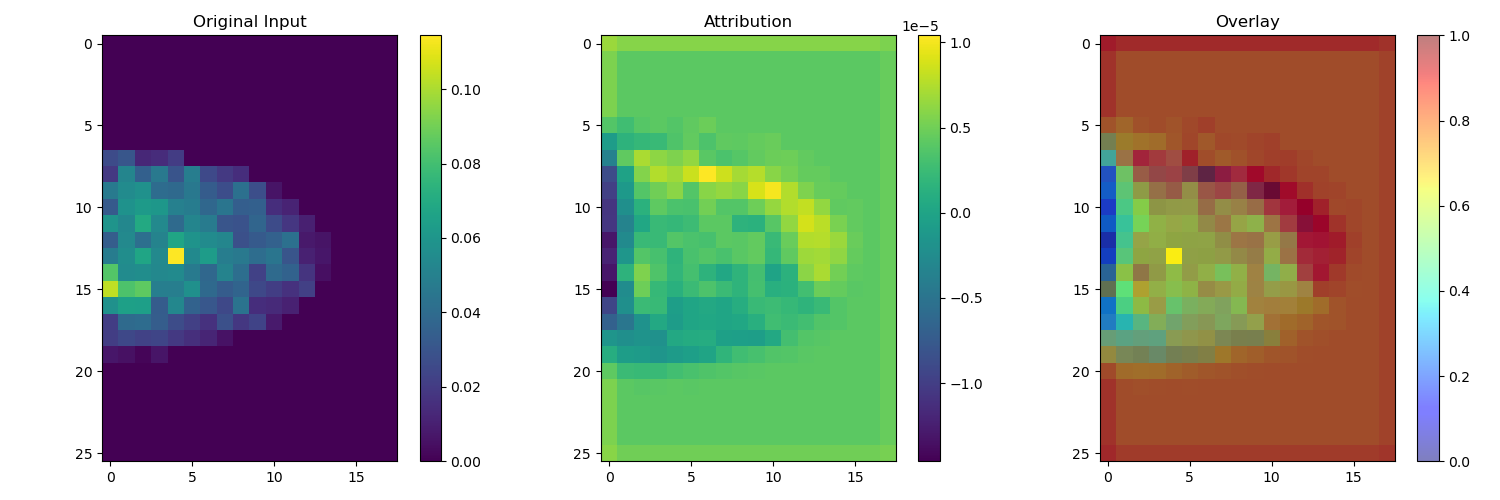
\includegraphics[width=1\textwidth]{attribution_overlay.png}
    \caption{Анализ первого блока UNet с помощью GradCAM}
    \label{gradU}
\end{figure}

\begin{figure}[H]
    \centering
    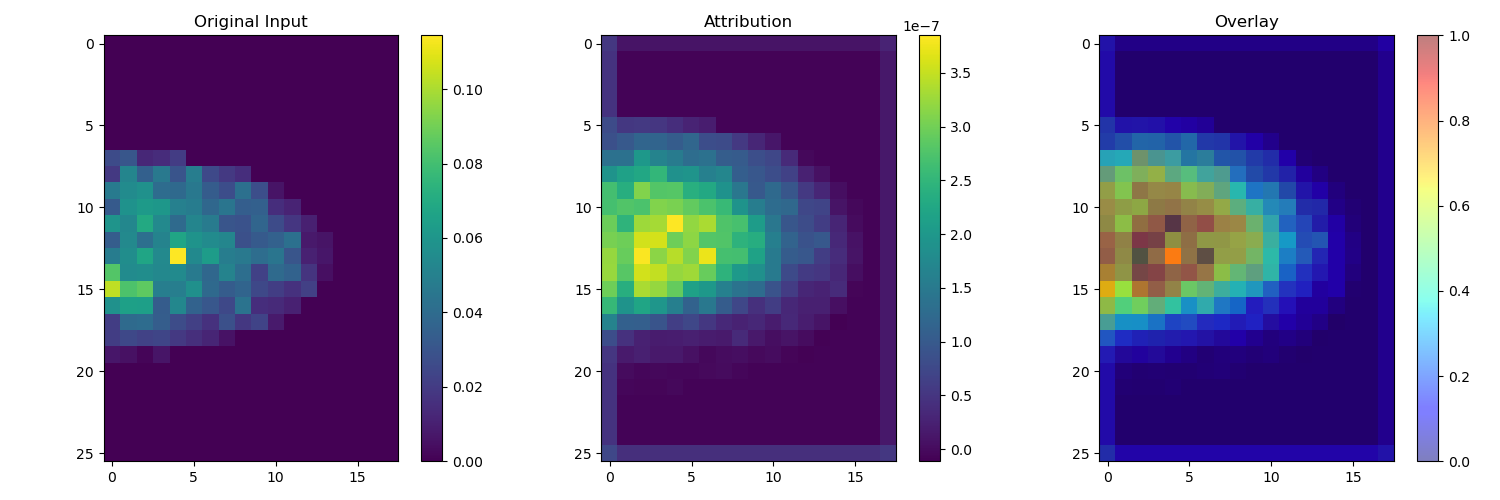
\includegraphics[width=1\textwidth]{attribution_overlay_fft.png}
    \caption{Анализ первого блока FFT\_UNet с помощью GradCAM}
    \label{gradFFT}
\end{figure}

Также были получены карты чувствительности для данных моделей (рис. \ref{sens}). По ним можно сделать вывод, что модели в целом робастные и стабильно работают при добавлении шума практически во всем обратном пространстве. Однако существуют единичные воксели, которые претерпевают большие возмущения из-за шума. 


\begin{figure}[H]
    \centering
    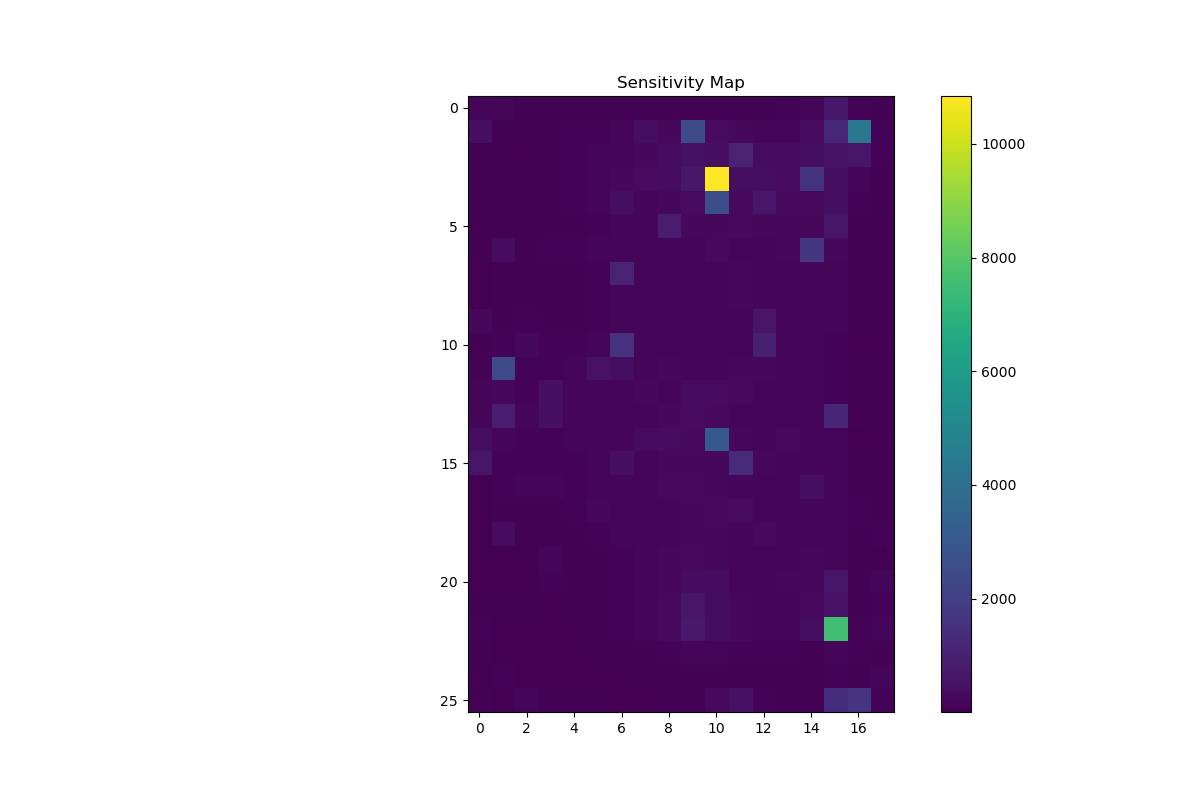
\includegraphics[width=0.5\textwidth]{sensitivity_map.png}\hfill
    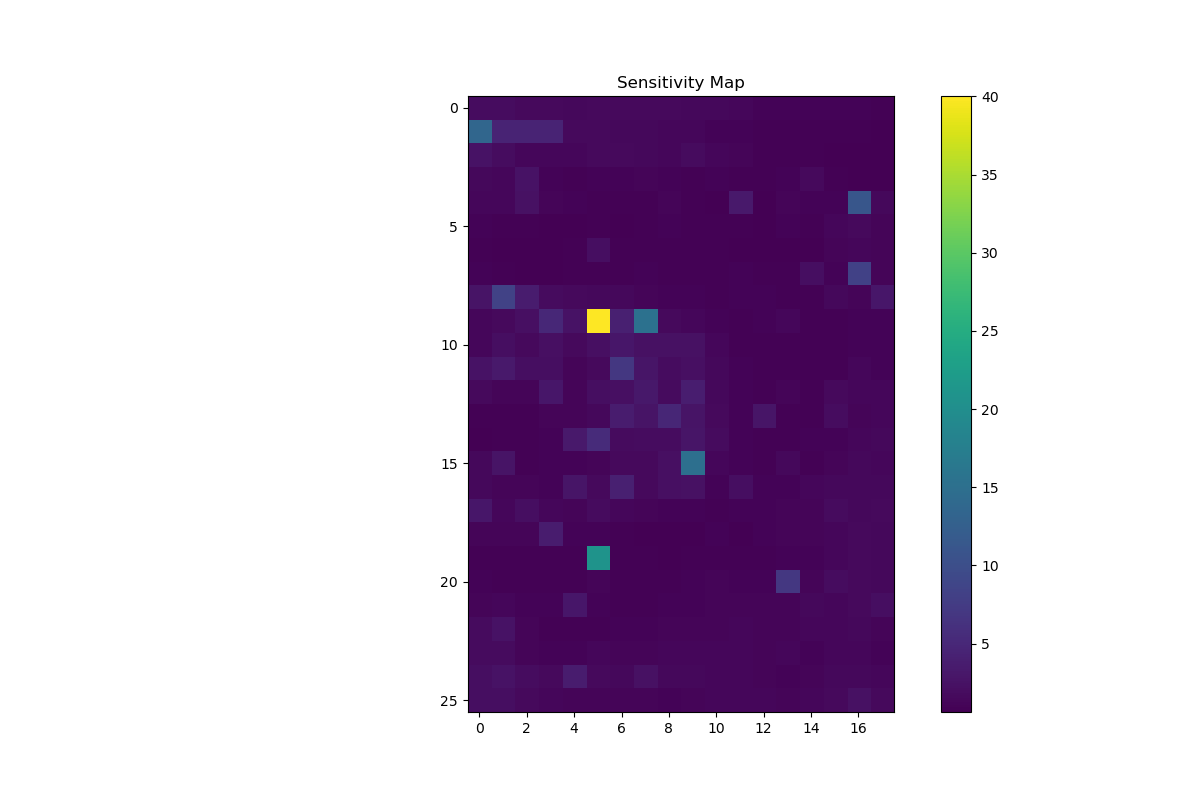
\includegraphics[width=0.5\textwidth]{sensitivity_map_fft.png}
    \caption{Карты чувствительности для UNet (слева) и FFT\_UNet (справа)}
    \label{sens}
\end{figure}





\subsubsection*{Проверка на реальных данных}

Несмотря на неплохие значения метрик на реальных моноклинных структурах из Кембриджского Банка Структурных данных, качества восстановления тензора отражений недостаточно для решения структуры с помощью SHELXT. На рис. \ref{recon_ex} представлены сечения тензора отражений для реальной структуры, R-фактор восстановленного тензора с помощью FFT\_UNet равен 0.346. Нейросеть достаточно точно предсказывает границы дифракционной картины, средние значения по вокселям (если их брать по дуге) тоже достаточно близки. Но восстановленные значения в тензоре более смазанны вдоль этих дуг, картине не хватает более точного распределения амплитуд по соседним вокселям в каждой локальной области. 

\begin{figure}[H]
    \centering
    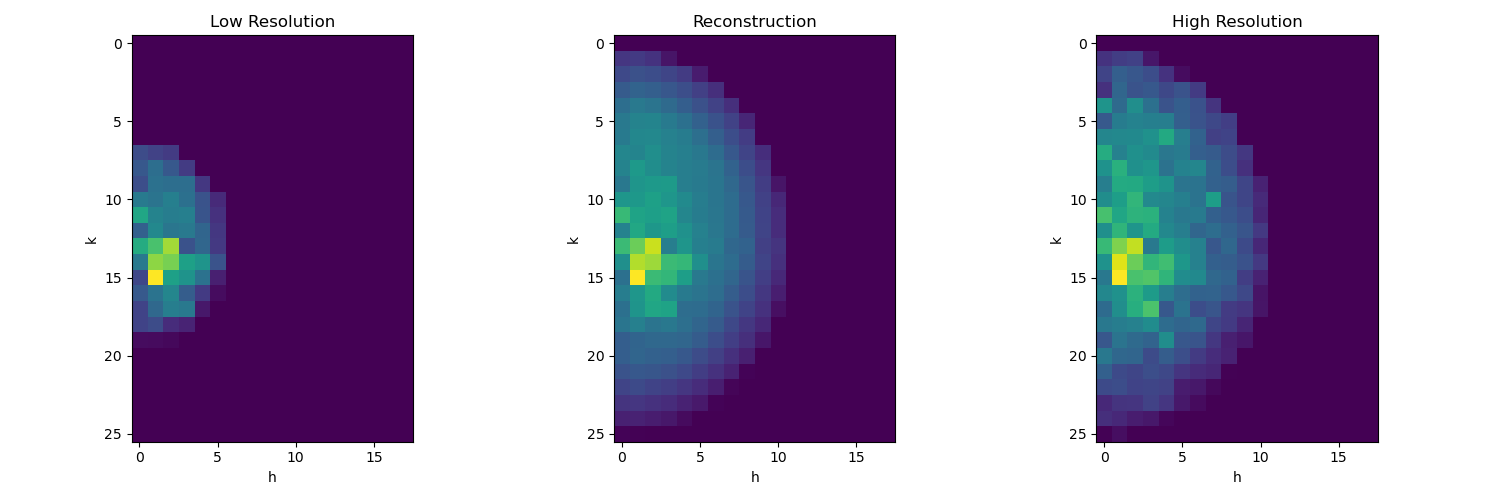
\includegraphics[width=1\textwidth]{recon_example.png}
    \caption{Типичная реконструкция дифракции реальной структуры, $R = 0.346$}
    \label{recon_ex}
\end{figure}

Как уже было оговорено, дифракционные отражения не обладают локальной связанностью, и для успешного решения задачи фаз требуется очень точно определить амплитуду в каждом вокселе. Несмотря на то, что модели машинного обучения успешно схватывают кристаллографические закономерности, им не хватает более точного численного определения в каждом вокселе данных. Таким образом, методы глубокого обучения успешно определяют кристаллографические паттерны и закономерности в обратном пространстве, однако им не хватает точности для решения проблемы фаз при восстановлении численных значений амплитуд отражений.

\subsubsection*{Дальнейшие планы и предложения}

В работе было показано, что методы ИИ успешно схватывают кристаллографические закономерности, однако из-за специфики обратного пространства для решения проблемы фаз им не хватает точности. Совершив переход в локально связанное пространство, можно предположить, что нейронные сети справятся с поставленной задачей.

Для решения проблемы фаз часто используется так называемая функция Паттерсона:

\begin{center}
    $P(u, v, w) = \sum\limits_{h,k,l\in Z} |F(h,k,l)|^2e^{-2\pi i(hu+kv+lw)}$
\end{center}

Таким образом, функция Паттерсона является Фурье-преобразованием интенсивностей дифракционных максимумов, где за их фазы приняты нули. Таким образом, перейдя от тензора амплитуд/интенсивностей к трехмерной картине функции Паттерсона --- получается классическая задача Super Resolution, поскольку для дифракционной картины низкого разрешения получится Фурье-образ низкого разрешения, разрешение которого требуется повысить так, чтобы восстановленная картина соответствовала Фурье-образу дифракционной картины высокого разрешения (рис. \ref{patt}). После увеличения разрешения трехмерной картины функции Паттерсона, мы можем вернуться в обратное пространство, рассчитав интенсивности (и из них амплитуды) рентгенодифракционных отражений, и решить проблему фаз с помощью уже описанных ab initio методов.

\begin{figure}[H]
    \centering
    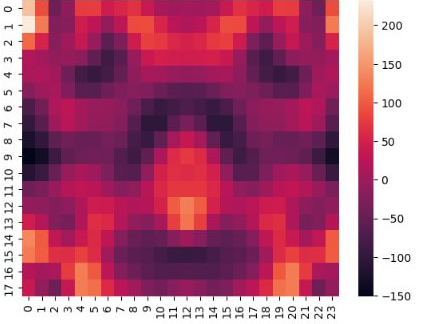
\includegraphics[width=0.5\textwidth]{patt_high.png}\hfill
    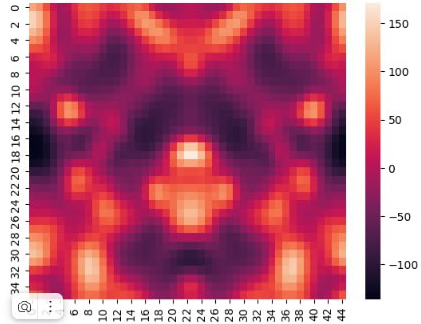
\includegraphics[width=0.5\textwidth]{patt_low.png}
    \caption{Типичное сечение функции Паттерсона по данным низкого (слева) и высокого (справа) разрешения}
    \label{patt}
\end{figure}

\subsection*{Выводы}

\begin{itemize}
\item Разработано программное обеспечение по генерации синтетических рентгенодифракционных данных, которое может быть использование для решения прикладных задач рентгеновской дифракции с помощью ИИ (\url{github.com/blackwood168/xrd_simulator})

\item Разработан единый пайплайн (\url{github.com/blackwood168/xrd_phase_ml}), позволяющий проводить воспроизводимые эксперименты по обучению, тестированию и inference задачи предсказывания дальних отражений по ближним для решения проблемы фаз

\item Разработаны и обучены на синтетических и реальных структурах UNet в качестве baseline, FFT\_UNet --- кастомный UNet с Фурье-преобразованием в слоях, XRD\_Transformer --- модель на основе трансформер со специфичным эмбеддингом, вписывающимся в физику задачи

\item Проведен анализ моделей, подтверждающий, что модели глубокого обучения выявляют кристаллографические закономерности и имеют потенциал решения прикладных задач рентгеновской дифракции

\item У моделей не достает качества численного восстановления рентгеновских отражений для решения проблемы фаз, несмотря на улавливание рентгенодифракционных паттернов; приведено обоснование и предложен план изменения методологии для решения задачи

\end{itemize}
}


\sloppy{
\addcontentsline{toc}{subsection}{Список литературы}
%\bibliographystyle{gost71s}
%\bibliographystyle{utf8gost705u}
%\bibliographystyle{utf8gost71s}
%\bibliographystyle{gost2008}
\bibliographystyle{gost2008l}
\bibliography{lit}

}
\end{document}
